% =====================================================================
% Supplementary Information
% What an SO(3) orientation flow can and cannot learn in
% molecular-crystal structure prediction
% =====================================================================
\documentclass[11pt]{article}
\usepackage[margin=1in]{geometry}
\usepackage{amsmath,amssymb,booktabs,microtype}
\usepackage{graphicx}
\usepackage[numbers,super,sort&compress]{natbib}
\usepackage[colorlinks=true,allcolors=blue]{hyperref}

\renewcommand{\thesection}{S\arabic{section}}
\renewcommand{\thetable}{S\arabic{table}}
\renewcommand{\thefigure}{S\arabic{figure}}

\title{\bfseries Supplementary Information:\\
What an SO(3) orientation flow can and cannot learn in
molecular-crystal structure prediction}
\author{Frank Cai}
\date{}

\begin{document}
\maketitle

% =====================================================================
\section{Method validation on single-block inorganic benchmarks}
% =====================================================================

The orientation analysis in the main text isolates a target obstruction that is
specific to multi-copy molecular crystals. To confirm that the underlying
SymMC-Flow architecture, training objective, and Runge--Kutta sampler are sound
independently of that obstruction, we benchmarked the model on two standard
single-block datasets, carbon-24 and MP-20, in which each atom is its own rigid
block and the orientation head is inactive ($\lambda_{\text{orient}}=0$). These
results are reported for completeness; they are not the contribution of this
paper.

\paragraph{Protocol.} We compare against joint equivariant
diffusion\cite{jiao2023diffcsp} using its released models, with matched
evaluation: $256$ held-out targets, $20$ samples per target, and the same
root-mean-square structure distance routine for both methods. Match rate at $k$
(``match@$k$'') is the fraction of targets for which at least one of $k$ samples
matches the reference under StructureMatcher\cite{ong2013pymatgen}. SymMC-Flow
samples in $50$ Runge--Kutta steps, against roughly $1{,}000$ steps for the
diffusion baseline.

\paragraph{Outcome.} Table~\ref{tab:inorganic} shows a mixed result: each method
wins two of the four match cells. SymMC-Flow leads on carbon-24 match@1 and on
MP-20 match@20, while the diffusion baseline leads on MP-20 match@1 and on
carbon-24 match@20 and produces tighter RMSE on matched structures. The honest
summary is that SymMC-Flow is competitive at roughly an order of magnitude fewer
sampling steps, not a uniform improvement. This is sufficient to establish that
the flow and sampler are well-behaved, which is all the main-text analysis
requires.

\begin{table}[h]
\centering
\caption{SymMC-Flow versus a diffusion baseline\cite{jiao2023diffcsp} on
single-block inorganic CSP under a matched evaluation ($256$ targets, $20$
samples, identical RMSD routine). Match rates in percent; higher is better. Each
method wins two of the four cells.}
\label{tab:inorganic}
\begin{tabular}{llcc}
\toprule
dataset & metric & SymMC-Flow & diffusion baseline \\
\midrule
carbon-24 & match@1  & \textbf{26.7} & 18.8 \\
carbon-24 & match@20 & 79.7 & \textbf{89.1} \\
MP-20     & match@1  & 41.4 & \textbf{48.0} \\
MP-20     & match@20 & \textbf{80.5} & 76.2 \\
\bottomrule
\end{tabular}
\end{table}

\paragraph{Caveat on benchmarks.} Recent work shows that carbon-24 contains a
large fraction of duplicate structures and that match-rate metrics can mislead
when identical building blocks exhibit structural
variety\cite{martirossyan2025matching}. The numbers above should be read as a
sanity check on the architecture under the field's conventional protocol rather
than as a definitive ranking.

% =====================================================================
\section{Is the absolute molecular orientation uniform on SO(3)?}
% =====================================================================

The main-text claim that the free asymmetric-unit pose $R_{\text{asym}}$ carries
no learnable signal predicts that the absolute per-molecule orientations should be
close to Haar-uniform on $\mathrm{SO}(3)$, since a uniform target offers nothing to
predict. For Haar-uniform rotations the geodesic angle $\theta$ from the identity
has density $p(\theta)=(1-\cos\theta)/\pi$ on $[0,\pi]$, with mean $126.5^\circ$.
Figure~\ref{fig:rasym} compares the empirical distribution of the reference-copy
orientations, which equal $R_{\text{asym}}$ up to the operation generating the
first-detected copy, to this density. The empirical distribution tracks the Haar
curve across the full angular range, with mean $122.6^\circ$ ($n=1{,}467$). A
one-sample Kolmogorov--Smirnov test against the Haar law gives $D=0.04$, a small
but nonzero deviation localized to a near-identity excess that comes from the
gauge-defining copies, whose self-alignment lands near the identity. The absolute
orientation is therefore close to uniform, consistent with the predict-zero floor,
and the residual deviation is a gauge artifact rather than a broad packing
preference.

\begin{figure}[h]
\centering
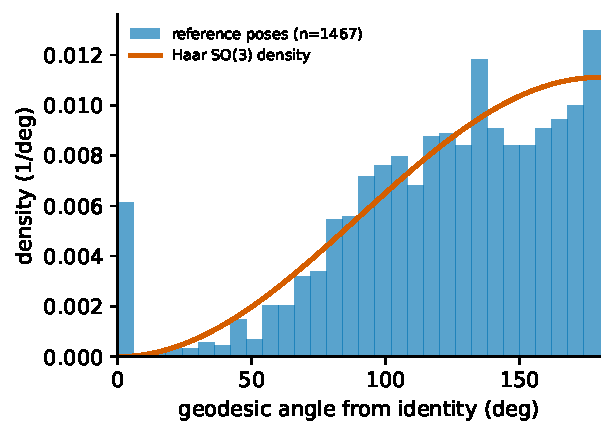
\includegraphics[width=0.62\linewidth]{figures/figS_rasym.pdf}
\caption{Empirical distribution of absolute reference-copy orientations (geodesic
angle from the identity) against the Haar-uniform $\mathrm{SO}(3)$ density. The two
agree across the range apart from a small near-identity excess from gauge-defining
copies.}
\label{fig:rasym}
\end{figure}

% =====================================================================
\section{Is $R_{\text{asym}}$ \emph{conditionally} predictable from packing?}
% =====================================================================

The uniformity test of the previous section concerns the \emph{marginal}
distribution of $R_{\text{asym}}$. A uniform marginal is necessary but not
sufficient for the operational claim that packing carries no signal about the
free pose: a weak conditional dependence
$p(R_{\text{asym}}\mid\text{packing})$ can coexist with a Haar marginal once the
packing is marginalized out. We therefore test the conditional directly with a
supervised probe. For each species we form a feature vector from the lattice cell
parameters, the molecule's fractional centroid, the mean and spread of all
centroids in the cell, the conformer's intrinsic shape (the gyration-tensor
eigenvalues), the molecule and atom counts, and a learned space-group embedding,
and we train a three-layer network to regress the reference-copy orientation
(a continuous six-dimensional rotation parametrization with a Frobenius loss).
The probe sees only composition and packing; the orientation is never an input.

Table~\ref{tab:probe} reports the held-out geodesic error against two references:
the single best feature-free predictor, which is the Fr\'echet (chordal) mean of
the training orientations, and a random-rotation guess. Averaged over three
splits the probe attains $125.2^\circ$, which does not improve on the
feature-free constant at $122.4^\circ$ and is statistically indistinguishable from
the random-guess level of $123.5^\circ$; the probe's mean ``improvement'' over the
constant is $-2.4\%$, i.e.\ no improvement. The network can drive its training
error well below these values, so the failure is one of generalization, not of
capacity. The conditional test thus reaches the same conclusion as the marginal
one by an independent route: under the composition-and-packing conditioning
available here, $R_{\text{asym}}$ is not predictable, which is the precise,
operational sense in which we call it unlearnable.

\begin{table}[h]
\centering
\caption{Conditional-predictability probe for $R_{\text{asym}}$: held-out mean
geodesic error (degrees, mean over three splits; lower is better). The probe,
given composition and packing, does not beat the feature-free constant and sits
at the no-information level.}
\label{tab:probe}
\begin{tabular}{lc}
\toprule
predictor & held-out geodesic error \\
\midrule
random guess (no information)        & $123.5^\circ$ \\
constant (Fr\'echet mean, feature-free) & $122.4^\circ$ \\
probe (composition + packing features)  & $125.2^\circ$ \\
\bottomrule
\end{tabular}
\end{table}

% =====================================================================
\section{StructureMatcher tolerance sweep for the orientation-isolated rate}
% =====================================================================

The main-text reconstruction rate uses a length tolerance of $0.3$, a site
tolerance of $0.5$, and an angle tolerance of $10^\circ$. To show the result is
not an artifact of that choice, Table~\ref{tab:sweep} sweeps the three
StructureMatcher tolerances on a representative trained checkpoint, reporting both
a single deterministic draw (match@1) and the best of eight draws (match@8). The
match decision uses \texttt{StructureMatcher.fit} (maximum atomic displacement
$\leq$ the site tolerance), the same strict criterion as the headline; the median
root-mean-square displacement is computed only over structures that already pass.
The rate rises monotonically from $5.3\%$ at the tightest setting to $20.6\%$ at
the loosest, while the oracle that uses the true orientation matches every
structure at all four settings, confirming the tolerances are not so loose as to
admit spurious matches. The default row ($0.3/0.5/10^\circ$) gives $16.0\%$
match@8 on this checkpoint; the main-text $13.7\pm2.0\%$ is the mean over three
independent training seeds at this row.

\begin{table}[h]
\centering
\caption{Orientation-isolated reconstruction under a StructureMatcher tolerance
sweep (single trained checkpoint; $n=131$ held-out multi-copy crystals; true
lattice, centroid, and conformer; only $\mathrm{SO}(3)$ sampled). The oracle
matches every structure at every setting. Match decided by
\texttt{StructureMatcher.fit}; RMSD is over matched structures only.}
\label{tab:sweep}
\begin{tabular}{ccccccc}
\toprule
$\ell$tol & stol & angle & match@1 & match@8 & med.\ RMSD (\AA) & oracle match@8 \\
\midrule
0.20 & 0.20 & $8^\circ$  & $0.0\%$ & $5.3\%$  & $0.089$ & $100\%$ \\
0.30 & 0.30 & $10^\circ$ & $1.5\%$ & $9.9\%$  & $0.113$ & $100\%$ \\
0.30 & 0.50 & $10^\circ$ & $3.8\%$ & $16.0\%$ & $0.128$ & $100\%$ \\
0.50 & 0.70 & $15^\circ$ & $4.6\%$ & $20.6\%$ & $0.142$ & $100\%$ \\
\bottomrule
\end{tabular}
\end{table}

% =====================================================================
\section{Leakage-controlled species-grouped split}
% =====================================================================

Because a single conformer registry is shared across crystals, a random
train/validation split could place two crystals of the same species on opposite
sides, raising the concern that the learnable relative-orientation signal reflects
species memorization rather than transferable geometry. We rule this out with a
species-grouped split (Methods): crystals sharing any species are grouped by
union--find and whole groups are assigned to one side, so no species crosses the
partition. Table~\ref{tab:grouped} compares the held-out non-reference
orientation drop under the two split regimes over three seeds. The grouped split
gives $28.5\pm2.9\%$, statistically indistinguishable from the random-split
$27.5\pm2.7\%$, so the effect is not species leakage. An orientation-isolated
reconstruction read on the grouped split (seed 0) recovers $10.7\%$ of held-out
crystals (match@8; $4.6\%$ match@1; median RMSD $0.140$~\AA) against $0\%$ for the
predict-floor field, confirming the reconstruction also survives the leakage
control.

\begin{table}[h]
\centering
\caption{Held-out non-reference orientation drop under random versus
species-grouped train/validation splits (three seeds each, mean $\pm$ s.d.). The
grouped split eliminates shared-species overlap; the signal is unchanged.}
\label{tab:grouped}
\begin{tabular}{lc}
\toprule
split & non-reference drop \\
\midrule
random (main text)        & $27.5\pm2.7\%$ \\
species-grouped (no leakage) & $28.5\pm2.9\%$ \\
\bottomrule
\end{tabular}
\end{table}

% =====================================================================
\section{All-atom de-novo baseline}
% =====================================================================

To place the $0\%$ end-to-end rigid-body result in context, we trained an
all-atom control that discards the rigid-body factorization: every atom is its own
block and the orientation head is disabled ($\lambda_{\text{orient}}=0$), the
representation used by all-atom molecular-crystal
generators\cite{jin2025oxtal,subramanian2026packflow}. It is trained on the same
$964/131$ split and evaluated for de-novo reconstruction (all manifolds sampled
from the prior) against both a random-prior floor and the trained field, with
match@20 best-of-twenty draws. Its lattice and centroid heads train normally (an
$88\%$ drop in flow-matching loss over $8{,}000$ steps), yet it reconstructs no
held-out crystal exactly: match@1 and match@20 are both $0\%$ (Wilson $95\%$ CI
$0$--$2.8\%$, $n=131$), identical to the random-prior floor
(Table~\ref{tab:allatom}). End-to-end molecular-crystal reconstruction at this
corpus scale is therefore out of reach for the all-atom representation as well, so
the $0\%$ reported for rigid-body generation reflects the corpus scale and compute
budget rather than a deficiency unique to the rigid-body factorization. This is
our own all-atom flow at the thousand-crystal scale, not one of the published
all-atom generators\cite{jin2025oxtal,subramanian2026packflow} trained on far
larger corpora; it isolates the effect of the representation at a fixed scale and
makes no claim about those larger models.

The best-of-twenty packing-component errors confirm the failure is the same joint
packing that bottlenecks the rigid-body model, not a representation-specific
pathology: the trained all-atom flow leaves a median lattice-parameter error of
$0.33$ and a median fractional-coordinate error of $0.46$ (Table~\ref{tab:allatom}),
comparable to the rigid-body de-novo errors reported in the main text (lattice
$0.46$, centroid $0.35$). Both representations place molecules roughly a third to a
half of a cell from their true positions, which is why neither reconstructs a
crystal exactly.

\begin{table}[h]
\centering
\caption{De-novo all-atom reconstruction on $131$ held-out crystals (all manifolds
sampled, best of twenty draws). The trained all-atom flow does not beat its
random-prior floor at this corpus scale, despite its packing heads training
normally, and its best-of-twenty packing errors match the rigid-body model's.}
\label{tab:allatom}
\begin{tabular}{lcccc}
\toprule
field & match@1 & match@20 & med.\ lattice-param & med.\ frac.\ coord. \\
\midrule
random prior (floor)   & $0.0\%$ & $0.0\%$ & --- & --- \\
trained all-atom flow  & $0.0\%$ & $0.0\%$ & $0.33$ & $0.46$ \\
\bottomrule
\end{tabular}
\end{table}

\bibliographystyle{unsrtnat}
\bibliography{references}

\end{document}
